
%In low-temperature plasmas (LTPs), electrons often deviate from the Maxwell-Boltzmann (Maxwellian) distribution. An accurate representation of the electron distribution function (EDF) is critical for accurate LTP modeling. Representing such non-Maxwellian distribution functions requires one to solve the Boltzmann transport equation (BTE). 

This section presents an overview of the electron BTE (see \Cref{subsec:bte}) and its application to model electron transport in glow discharge devices (see \Cref{subsec:glow_discharge}). 
\Cref{tab:summary_symbols} summarizes the symbols used in the paper. 
%presents symbols used in this paper and their descriptions.
\begin{table}[!tbhp]
	\centering
	\resizebox{0.9\textwidth}{!}{
		\begin{tabular}{||c|p{6cm}|c|p{7cm}||}
			\hline
			\hline
			Symbol & Description 	&		Symbol & Description\\
			\hline
			$p_0$    & \small Gas pressure 	  & $T_0$    & \small Gas temperature\\
			$n_0$    & \small Neutral density & $L  $    & \small Electrode gap \\
			$V_0$    & \small Peak voltage    & $\zeta  $    & \small Oscillation frequency\\
			$D_e$    & \small Electron diffusion coefficient & $D_i$    & \small Ion diffusion coefficient \\
			$\mu_e$  & \small Electron mobility coefficient & $\mu_i$  & \small Ion mobility coefficient \\
			$T_e$    & \small Electron temperature & $q_e$    & \small Electron charge\\
			$m_e$    & \small Electron mass      & $f\of{\vect{x}, \vect{v}, t}$ & \small EDF \\
			$\vect{E}$ & \small Electric field   & $N_x$ & \small Number of collocation points in $x$\\ 
			$N_r$ & \small Number of B-splines in v & $N_\vtheta$ & \small Number of ordinates in $\vtheta$\\
			$N_l$ & \small Number of spherical harmonics in $\vtheta$ & $\vect{C}_{en}$ & \small Discrete electron-neutral collision operator \\ 
			$\vect{A}_v$ & \small Discrete velocity space advection & $\vect{D}_x$ & \small Spatial derivative operator (Chebyshev-collocation)\\
			$\vect{A}_x$ & \small Galerkin projection of $v \cos(\vtheta) \nabla_{\vect{x}} f$ term & $\vect{P}_S$ & \small $\vtheta$ ordinates to spherical harmonics projection \\
			$\vect{P}_O$ & \small Spherical harmonics to $\vtheta$ ordinates projection & $\vect{F}$ & \small Discretized EDF \\
			$\sigma_{0}$ & \small Momentum transfer cross-section & $\sigma_{i}$ & \small Ionization cross-section \\
			\hline
			\hline
	\end{tabular}}
	\caption{Notation \label{tab:summary_symbols}}
\end{table}
\subsection{The electron Boltzmann transport equation (BTE)}
\label{subsec:bte}
The electron BTE driven by an electric field $\vect{E}\of{\vect{x}, t}$ is given by
\begin{equation}\label{eq:bte-full}
	\partial_t f + \vect{v} \cdot \nabla_{\vect{x}} f- \frac{q_e \vect{E}}{m_e} \cdot \nabla_{\vect{v}} f = C_{en}(f).
\end{equation} Here, $f\of{\vect{x}, \vect{v}, t}$ denotes the EDF, $\vect{x} \in \Omega \subset \reals^3$, $\vect{v}\in \reals^3$ and $t\in \reals$, and $C_{en}$ denotes the electron-heavy  binary collision operator. %The evolution of the EDF is governed by the integro-differential Boltzmann equation given by \Cref{eq:bte-full}. In \Cref{eq:bte-full} the left-hand side (LHS) denotes the spatial advection (i.e., $\vect{v} \cdot \nabla_{\vect{x}} f$) velocity space acceleration (i.e., $\frac{q_e \vect{E}}{m_e} \cdot \nabla_{\vect{v}} f$),  and the right-hand side denotes the electron-heavy binary collisions, e.g., elastic, ionization. 
$C_{en}$ compromises the electron-heavy momentum transfer and ionization collisions and $f\of{\vect{x}, \vect{v}, t} d\vect{x} d\vect{v}$ denotes the number of electrons for the phase-space volume $d\vect{x} d\vect{v}$. Using spherical coordinates $\vect{v}=\of{v, \vtheta, \vphi}$ in velocity space and aligning the velocity space z-axis to $\vect{E}$ direction, we obtain $\vect{E} = E \vect{\hat{e}_z} = E \of{\cos(\vtheta) \vect{\hat{e}_r} - \sin(\vtheta)\vect{\hat{e}_\theta}}$. By restricting $\vect{x}$ in 1D, we obtain the 1D3V BTE which is given by
% The 1D BTE is given by 
%we can write the 1D-space Boltzmann equation as in \Cref{eq:bte-1d}.
\begin{equation}
    \text{[1D3V]:} \quad \partial_t f + v\cos\of{\vtheta} \partial_x f- \frac{q_e E}{m_e} \of{\cos(\vtheta) \partial_v f - \sin(\vtheta) \frac{1}{v} \partial_{\vtheta}f } = C_{en}(f). \label{eq:bte-1d}
\end{equation}
Furthermore, if we drop the spatial dependence entirely, we obtain the homogeneous 0D3V case, which is given by
\begin{equation}
	\text{[0D3V]:} \quad \partial_t f - \frac{q_e E}{m_e} \of{\cos(\vtheta) \partial_v f - \sin(\vtheta) \frac{1}{v} \partial_{\vtheta}f } = C_{en}(f). \label{eq:bte-0d}
\end{equation}

\par \textbf{Electron-heavy collisions}: The electron-heavy collision operator $C_{en}$ captures the rate of change in the EDF due to collisions. It is given by 
%\begin{multline}
%	C^{-}_{en}(f,f_0) = 
%	\qquad\myint_{\reals^3} \myint_{\reals^3} \myint_{S^2} 
%	B\of{\vect{v}_e^\prime, \vect{v}_0^\prime, \vect{\omega}} 
%	f\of{\vect{v}_e^\prime} f_0\of{\vect{v}_0^\prime} 
%	\delta\of{\vect{v}_e^\prime - \vect{v}_e} 
%	\diff{\vect{v}_0^\prime} \diff{\vect{v}_e^\prime} \diff{\vect{\omega}}, \label{eq:c_en_loss}
%\end{multline}
\begin{align}
	&C^{-}_{en}(f,f_0) =\myint_{\reals^3} \myint_{\reals^3} \myint_{S^2} 
	B\of{\vect{v}_e^\prime, \vect{v}_0^\prime, \vect{\omega}} 
	f\of{\vect{v}_e^\prime} f_0\of{\vect{v}_0^\prime} 
	\delta\of{\vect{v}_e^\prime - \vect{v}_e} 
	\diff{\vect{v}_0^\prime} \diff{\vect{v}_e^\prime} \diff{\vect{\omega}}, \label{eq:c_en_loss}
	\\
	&C^{+}_{en}\of{f,f_0} =\myint_{\reals^3} \myint_{\reals^3} \myint_{S^2} 
	B\of{\vect{v}_e^\prime, \vect{v}_0^\prime, \vect{\omega}} 
	f\of{\vect{v}_e^\prime} f_0\of{\vect{v}_0^\prime} 
	\delta\of{\vect{v}_e^\text{post}\of{\vect{v}_e^\prime, \vect{v}_0^\prime, \vect{\omega}} - \vect{v}_e} 
	\diff{\vect{v}_0^\prime} \diff{\vect{v}_e^\prime} \diff{\vect{\omega}} \label{eq:c_en_gain},\\
	&C_{en}\of{f,f_0} = \qquad C^{+}_{en}\of{f,f_0} - C^{-}_{en}\of{f,f_0} \label{eq:c_en}.
\end{align} Here, $f_0$ denotes the heavy species distribution function, and $B$ denotes the probability measure for a given collision parameters. The collision kernel $B$ is defined by the collision cross-section~\cite{pitchford2017lxcat}. These expressions can be further simplified by using the following common to LTPs assumptions: 1) The heavy species distribution functions are Maxwellian, and 2) electron-heavy collisions follow isotropic scattering. Here, the isotropic scattering assumption ensures that the collision probability measure is independent of the scattering angle. Under these assumptions, the BTE preserves the azimuthal symmetry in the velocity space. \Cref{eq:c_en} can be further simplified by assuming Maxwellian distribution for heavy species, i.e., $f_{0}\of{\vect{v}} = \frac{n_0}{\of{\sqrt \pi v_{th,0}}^3} \exp\of{\of{-v/v_{th,0}}^2}$ where $v_{th,0}=\sqrt{2k_B T_0/m_0}$ is the thermal velocity, $n_0$ is the number density, and $m_0$ is the mass of the heavy species.      

% \textbf{Electron-heavy collisions}: In \Cref{eq:bte-1d}, $C_{en}$ denotes the integral operator capturing the binary collisions between electrons and background gas particles. 
\subsection{Glow discharge}
\label{subsec:glow_discharge}
Here, we summarize the formulation for RF-GDPs. An externally imposed potential difference between two electrodes at the opposite ends of a tube filled with argon is used to generate a plasma. \Cref{fig:glow_schematic} shows a schematic of the glow discharge device. 
\begin{figure}[!tbhp]
    \centering
    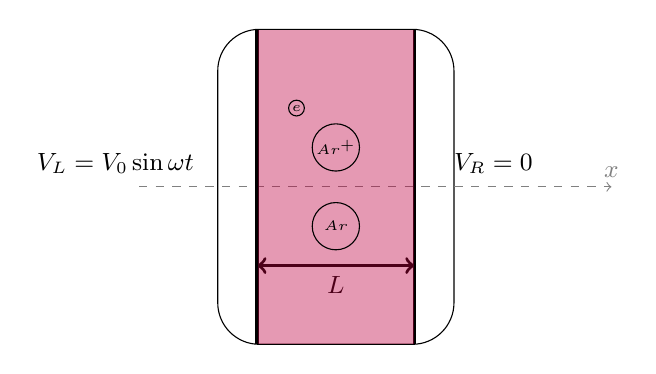
\begin{tikzpicture}
        \draw[rounded corners=15pt]   (0,0) rectangle ++(3,4);
        \draw[->, dashed, gray]   (-1,2) -- (5,2) node[above] {\small $\vect{x}$};
        \draw[-,black, very thick]   (0.5,0)--(0.5,4) node at (-1.3, 2.3) {\small $V_L=V_0\sin\of{\omega t}$};
        \draw[-,black, very thick]   (2.5,0)--(2.5,4) node at ( 3.5, 2.3) {\small $V_R=0$};
        \draw[<->,black, very thick]   (0.5,1)  --(2.5,1) node[below, xshift=-1cm] {\small $L$};
        \draw[fill=purple, fill opacity=0.4]   (0.5,0) rectangle ++(2.0,4);
        \draw (1.5,1.5) circle [radius=0.3] node {\tiny $Ar$};
        \draw (1.5,2.5) circle [radius=0.3] node {\tiny $Ar^{+}$};
        \draw (1.0,3.0) circle [radius=0.1] node {\tiny $e$};
        %\node (1) [draw, rounded rectangle] {rounded rectangle};
    \end{tikzpicture}
    \caption{An illustrative schematic for the glow discharge plasma with Argon. \label{fig:glow_schematic}}
\end{figure}
The imposed potential generates an electric field that causes electron acceleration and ionization of the background heavy species, which results in the glow discharge plasma. Following standard approximations for GDPs, our formulation is based on the following assumptions:
%The following assumptions are made for the mathematical models used in this work to model the glow discharge phenomenon. 
\begin{enumerate}
    \item We assume the size of the electrodes is larger than the discharge length ($L$). Hence, discharge characteristics vary along the normal direction to electrodes.
    \item We limit our study to the three-species collisional model described in \Cref{t:col_list}. We only consider direct ionization from the neutral state, ignoring excitation and step-ionization from metastable states. We remark that our solver easily extends to more species and collision types. Furthermore, assuming constant $n_0(x, t)=n_0$ value, we only track ions and electrons. 
    \item We assume heavies have constant temperature $T_0$, typically the room temperature.  %\todo{do we need to mention on constant neutral density ? }
    \item Following~\cite{liu2014numerical}, we assume zero secondary electron emission from the electrode surface. 
\end{enumerate}
\begin{table}[!tbhp]
	\centering
	\begin{tabular}{|c|c|c|}
		\hline 
		Collision & Threshold & Post-collision\\
		\hline 
		$e + Ar \rightarrow e + Ar$ & None & $\varepsilon_{\text{post}} =\varepsilon_{\text{pre}}(1- \frac{2m_e}{m_0})$\\
		\hline
		$e + Ar \rightarrow Ar^{+} + 2e$ & $\varepsilon_{ion}$=15.76eV &  $\varepsilon_{\text{post}}=0.5 \of{\varepsilon_{\text{pre}}-\varepsilon_{\text{ion}}}$\\     
		\hline
	\end{tabular}
	\caption{Three species Ar collisional model. \label{t:col_list}}
\end{table}
We consider two formulations: In~\Cref{subsubsec:fluid_only}, we give a species transport formulation for the fluid approximation for both electrons and ions. In~\Cref{subsubsec:hybrid}, we give the hybrid approximation where the fluid approximation describes ions, and the BTE models the electron transport. As mentioned, we assume constant neutral species density and temperature in both cases.    
\subsubsection{Fluid model for electrons and ions}
\label{subsubsec:fluid_only}
We use a standard self-consistent fluid model for glow discharge phenomena~\cite{panneer2015computational,liu2014numerical}. The species number density continuity equations are given by 
\begin{subequations}
	\begin{align}
		&\partial_t{n_{e}} + \nabla \cdot \vect{J_e} = k_i n_0 n_e, \label{eq:fl_mass_continuity_ne}\\
		&\partial_t{n_{i}} + \nabla \cdot \vect{J_i} = k_i n_0 n_e. \label{eq:fl_mass_continuity_ni}
	\end{align}\label{eq:fl_mass_continuity}
\end{subequations}
\Cref{eq:fl_mass_continuity_ne,eq:fl_mass_continuity_ni} describe the evolution of ions and electron number densities where $k_i$ denotes the ionization rate coefficient, $n_0$ denotes the background neutral number density, and $n_e$ denotes the electron number density.  
%\begin{equation}
%    \partial_t{n_{k}} + \nabla \cdot \vect{J_k} = \dot{S}_k. \label{eq:fl_mass_continuity}
%\end{equation}
In \Cref{eq:fl_mass_continuity}, flux terms, $\vect{J}_{e}$ and $\vect{J}_{i}$ are approximated using a drift-diffusion approximation~\cite{hill1986introduction} and are given by 
\begin{equation}
	\vect{J}_e = -\mu_e n_e \vect{E} -D_e \nabla n_e \text{  and  } \vect{J}_i = \mu_i n_i \vect{E} -D_i \nabla n_i \label{eq:drift_diffusion_flux}.
\end{equation}
%In \Cref{eq:fl_mass_continuity_ne,eq:fl_mass_continuity_ni}, $\dot S_{e}$ and $\dot S_{i}$ denote the rate of production for electrons and ions. The above can be written as $\dot{S}_{e, i} = k_i n_0 n_e$, where $k_i$ denotes the ionization rate coefficient, $n_0$ denotes the background neutral number density, and $n_e$ denotes the electron number density.  
 
%Electrons undergo significant acceleration due to the electric field. The evolution of electron energy is prescribed by
The electron energy equation is given by 
\begin{equation}
	\partial_t \of{\frac{3}{2} n_e k T_e} = -\nabla \cdot \vect{q}_e - e \vect{J}_e \cdot \vect{E} - \varepsilon_{\text{ion}} k_i n_0 n_e \label{eq:fl_electron_energy} ,
\end{equation} and the electron energy flux term is specified by
\begin{equation}
	\vect{q_e} 	= -\frac{3 k D_e n_e}{2} \nabla T_e + \frac{5}{2} k T_e \vect{J_e} \label{eq:fl_e_energy_flux}.
\end{equation}

The underlying electric field potential is given by Gauss's law and given by
%specified by \Cref{eq:gauss_law}.
\begin{equation}
    \Delta V = -\frac{e}{\epsilon_0} (n_i-n_e) \text{ and } \vect{E} = - \nabla V \label{eq:gauss_law}.
\end{equation}
%%%%%%%%%%%%%%%%%%%%%%%%%%%%%%%%%%%%%%%%%%%%%%%%%%%%%%%%%%%%%%%%%%
\par \textbf{Boundary conditions}: For electrons, we enforce the Maxwellian flux boundary condition~\cite{panneer2015computational} given by
\begin{equation}
	\vect{J_e} \cdot \hat{\vect{n}} = \frac{1}{4} n_e \of{\frac{8k_B T_e}{\pi m_e}}^{0.5} \label{eq:e_flux_bc}, 
\end{equation} where $\hat{\vect{n}}$ is the outward unit normal vector. For the electron energy equation, the electron energy flux $\vect{q_e}$ at the boundary is enforced to the average energy each electron carry when it escapes from the discharge walls and given by $\vect{q_e} = \frac{5}{2} k_B T_e \vect{J_e}$. For the ions, the enforced boundary condition is given by
\begin{equation}
    \vect{J_i}\cdot \hat{\vect{n}} = - n_i \max(0, \mu_i \vect{E} \cdot \hat{\vect{n}}) \label{eq:fl_ion_bc}.
\end{equation} 
A Dirichlet condition for \Cref{eq:gauss_law} is given by the driving oscillatory voltage input
\begin{equation}
    V\of{x=0, t}=V_0 \sin\of{2\pi \zeta t} \text{ and } V\of{x=L, t} = 0 \label{eq:voltage_bc}.
\end{equation} 

The fluid approximation for the glow discharge problem requires the kinetic coefficients, $\mu_{e,i}$, $D_{e,i}$ and $k_i$. Following~\cite{liu2014numerical}, we use constant kinetic coefficients for the ions. For the electrons, we use temperature-based tabulated kinetic coefficients. \Cref{subsec:results_glowd} presents a detailed description of temperature-based electron kinetic coefficients. The fluid approximation for GDP simulation is summarized below. 
%\Cref{eq:fluid_model_eqs} summarizes the fluid model for glow discharge phenomena with the boundary conditions described above. 

\begin{subequations}
	\label{eq:fluid_model_eqs}
	\begin{empheq}[left={\forall t>0, x \in [0, L]\empheqlbrace}]{align}
			\partial_t n_i &= k_i(T_e) n_0 n_e - \nabla \cdot \vect{J_i} \label{e:fl_a},\\
			\partial_t n_e &= k_i(T_e) n_0 n_e - \nabla \cdot \vect{J_e} \label{e:fl_b},\\
			\partial_t \of{\frac{3}{2} n_e k T_e} &= -\nabla \cdot \vect{q}_e - e \vect{J_e} \cdot \vect{E} - \varepsilon_{\text{ion}} k_i(T_e) n_0 n_e \label{e:fl_c}, \\
			\vect{J}_i &=  \mu_i n_i \vect{E} -D_i \nabla n_i \label{e:fl_a_flux},\\
			\vect{J}_e &= -\mu_e\of{T_e} n_e \vect{E} -D_e\of{T_e} \nabla n_e\label{e:fl_b_flux},\\
			\vect{q_e} &= -\frac{3 k D_e\of{T_e} n_e}{2} \nabla T_e + \frac{5}{2} k T_e \vect{J_e}\label{e:fl_c_flux},\\
			\Delta V &= -\frac{e}{\epsilon_0} (n_i-n_e) \text{ , } \vect{E} = - \nabla V \label{e:fl_d}, 
	\end{empheq}
	\begin{empheq}[left={\forall t>0, x=0 \text{ and } x=L \empheqlbrace}]{align}
		& \vect{J_i}^\cdot \hat{\vect{n}} = - n_i \max(0, \mu_i \vect{E} \cdot \hat{\vect{n}}),\\
		& \vect{J_e} \cdot \hat{\vect{n}} = \frac{1}{4} n_e \of{\frac{8k_B T_e}{\pi m_e}}^{1/2} \label{e:fl_b_bdy},\\
		& \vect{q_e} = \frac{5}{2} k_B T_e \vect{J_e} \label{e:fl_c_bdy},\\
		&V\of{x=0, t}=V_0 \sin\of{2\pi \zeta t} \text{ , } V\of{x=L, t} = 0.
	\end{empheq}		
\end{subequations}

\subsubsection{Summary of the hybrid model}
\label{subsubsec:hybrid}
We replace Equations \eqref{e:fl_b}, \eqref{e:fl_c}, \eqref{e:fl_b_bdy}, and \eqref{e:fl_c_bdy}  with the 1D3V BTE. The combined equations become
%In the hybrid formulation, we use the fluid approximation for heavies and the BTE for electron transport. The overall hybrid model for the one-dimensional glow discharge problem is summarized by  
\begin{subequations}
	\label{eq:glow_hybrid}
	\begin{empheq}[left={\forall t>0, x \in [0, L]\empheqlbrace}]{align}
			& \partial_t{n_{i}} + \nabla \cdot \vect{J_{i}} = k_i n_0 n_e \label{eq:hybrid_cnt_a},\\
			&\partial_t f + v\cos\of{\vtheta} \partial_x f- \nonumber \\
			&\qquad\qquad\frac{q_e E}{m_e} \of{\cos(\vtheta) \partial_v f - \sin(\vtheta) \frac{1}{v} \partial_{\vtheta}f } = C_{en}(f) \label{eq:hybrid_cnt_b},  \\
			&\vect{J}_i =  \mu_i n_i \vect{E} -D_i \nabla n_i \label{eq:hybrid_cnt_a_flux},\\
			&k_i = \int_{\vect{v}} \norm{\vect{v}} \sigma_i \hat{f} \diff{\vect{v}} \text{ where } \hat{f}\of{\vect{v}} = \frac{f\of{\vect{v}}}{\int_{\vect{v}} f\of{\vect{v}} \diff{\vect{v}}}, \\
			& \Delta V = -\frac{e}{\epsilon_0} (n_i- n_e) \text{ , } \vect{E} = - \nabla V \label{eq:hybrid_cnt_c}, 
	\end{empheq} 
	\begin{empheq}[left={\forall t>0, x=0 \text{ and } x=L \empheqlbrace}]{align}
		& \vect{J_i}^\cdot \hat{\vect{n}} = - n_i \max(0, \mu_i \vect{E} \cdot \hat{\vect{n}}), \\
		& f(x=0, v, \vtheta \leq \frac{\pi}{2}, \vphi) = 0 \text{ and } \nonumber\\
		& \qquad\qquad f(x=L, v, \vtheta > \frac{\pi}{2}, \vphi) = 0 \label{eq:hybrid_cnt_b_bdy},\\
		& V\of{x=0, t}=V_0 \sin\of{2\pi \zeta t} \text{ , } V\of{x=L, t} = 0.
	\end{empheq}		
\end{subequations} Note that the EDF carries information on the electron number density $n_e(t,\vect{x}) = \int_{\vect{v}} f(t, \vect{x}, \vect{v}) \diff{\vect{v}}$ and $\sigma_i$ denotes the total ionization cross section and $\hat{f}$ denotes the normalized EDF. As prescribed above, we assume zero incoming flux boundary conditions for \Cref{eq:hybrid_cnt_b}.
